%\documentclass[11pt,epsf]{article}
%\documentstyle[12pt,amsmath]{article}
%\usepackage{html}
%\usepackage{epsf}
%\usepackage{amsmath}
%\usepackage[dvips]{graphicx, color}  % The figure package

%\setlength{\textheight}{23.0cm}
%\setlength{\textwidth}{15.00cm}
%\setlength{\topmargin}{-1.5cm}
%\setlength{\oddsidemargin}{1.5cm}
%\setlength{\evensidemargin}{1.5cm}
%\setlength{\parskip}{5pt}
%\setlength{\parindent}{20pt}

%\evensidemargin -0.7cm
%\oddsidemargin 1.5cm
%\textwidth 15cm
%\topmargin -1.5cm
%\textheight 23cm
\parskip 1ex    % White space between paragraphs amount

%\begin{document}
%\title{Benchmarking in AIPS++}
%\author{Sanjay Bhatnagar}
%\date{February 04, 2003}
%\maketitle

%\normalsize

%%%%%%%%%%%%%%%%%%%%%%%
\section{Introduction}
%%%%%%%%%%%%%%%%%%%%%%%

The purpose of this document is to describe the general approach for
benchmarking of AIPS++ and to initiate a focused discussion for
resolving performance issues in AIPS++.  The work done so far towards
this goal and the suite of benchmark tools developed in AIPS++ are
described.  The results available from the work so far, open questions
and ideas about where we should go from here are also discussed.

Some of the tools and techniques used for locating performance
bottle-necks in parts of AIPS++ are also described.  Some of these
probably have broader use in the project for quality assurance
purposes.  Appendix~\ref{A:PAGED_FFT} discusses the use of the FFTW
library and the possible interaction with the operating system
buffering which can have an impact on performance at large image sizes
and appendix~\ref{A:MEM_MODEL} discusses dynamic memory usage in
AIPS++.  Appendix~\ref{A:GPROF} describes the use of the GNU profiling
tools for AIPS++ applications.  Appendix~\ref{A:MEMUSAGE} provides a
script which can be used to effectively monitor the runtime memory
usage of an application and produce a memory usage profile.  Finally,
appendix~\ref{A:QUESTIONS} lists a few open questions.

{\it The performance curves and the tables in this document are for
the purpose of discussion.  Since optimization is an on-going activity
and is likely to remain so for a while, the latest progress reports of
this work is usually available from the AIPS++ Project Office on the
Internet.}\footnote{See {\tt
http://aips2.nrao.edu/projectoffice/imager.ps} and {\tt
http://aips2.nrao.edu/projectoffice/calibrater.ps}.}

%%%%%%%%%%%%%%%%%%%%%%%%%%%%%%%%%%%%%%%%%%%%%%%%%%%%%%%%%%%%%%%%%%%%%%%%%%%%%%%%%%%%
\section{Benchmarking of the {\tt imager} tool}
\label{IMAGER}
{\tt imager} is the primary imaging tool for interferometric data in
AIPS++.  The major data processing steps that are required to make an
astronomical image from a calibrated Visibility data stored in the
AIPS++ database format (the Measurement Set (MS)) are:

\begin{enumerate}

\item \underline{Make the PSF}: Grid the visibility weights on a regular
grid and invert them using FFT to make the Point Spread Function (PSF)
\label{MakePSF}

This involves reading the entire selected visibility database, which
is an I/O dominated operation.  The computational cost in this step
comes from the computations to put the visibility weights on the grid
and the FFT for inversion.  For a typical problem, both these are
comparatively inexpensive operations.  Hence, in general, the cost of
this step is dominated by the I/O efficiency of the system.  The I/O
itself is split between reading the MS and the paging of the complex
image (the grid).  The gridding algorithm used in AIPS++ goes into,
what is referred to as the {\it tiling mode}, if the complex image
size is greater than the image cache size in the memory.  The image
cache size and the tile size can both be set by the user.

In the {\it tiling mode}, the gridding algorithm uses the {\tt
LatticeCache} which holds a cache of image tiles used\footnote{Size of
this cache is same as that of the complex grid cache size, as set
using {\tt setoptions()}?}.  The algorithm attempts to utilize the
fact that not all parts of the uv-plane are populated and that the
uv-coverage is a slowly varying function of time.  Hence the algorithm
holds all tiles used in the gridding of the first integration time in
the Lattice cache.  Typically, for the next several integrations,
same set of tiles will be used from the cache, which will minimize the
I/O.  In the event of Lattice cache miss, a new tile is loaded from
the disk and simply added to the lattice cache.  If the cache is full,
space is made by over-writing the last-used tile in the cache.  This,
in some pathological cases, can be quiet inefficient.

%The cost of this step is therefore closely linked to the benchmark
%results of the Table system I/O (see Section~\ref{IOBenchmark}).

\item \underline{Make Dirty Image}: Grid the weighted visibilities on
      a regular grid and invert them using FFT to make the Dirty Image
      ($I^D$).
\label{MakeDI}

In terms of computing and I/O costs, this step is essentially same as
step \ref{MakePSF}\footnote{Are there significant extra cost
associated with co-ordinate conversion here?}.  The images (complex
and real) are represented by {\tt TempLattice} and depending upon the
image size and the available cache size, they are either disk based or
entirely in the memory.

\item \underline{Deconvolution}: Make a sky model image ($I^M$) by
      deconvolving the effects of the PSF  from the dirty image.  This
      solves the equation $I^D = I^M\star PSF$ for $I^M$.
\label{MakeIM}

This step involves use of one of the many deconvolution algorithms
implemented in AIPS++.  Since each of these algorithms are
significantly different - both in compute and I/O cost, these need to
be analyzed and benchmarked separately.  Here, we discuss only the
single field Clark-Clean (SFCC) algorithm\footnote{See {\tt
http://aips2.nrao.edu/projectoffice/imager.ps} for performance curves
of the Cotton-Schwab variant of the algorithm.}.

SFCC works in two cycles, referred to as the major and minor cycles.
In the minor cycle, a Clean-component (CC) list is generated by
deconvolving an approximate PSF, till this process runs out of
accuracy (and starts diverging).  At this point, a major cycle is
invoked which computes a model visibility ($V^M$) using the CCs and
reconciles them with the calibrated visibilities ($V$).  A residual
image is then computed by inverting the residual visibilities
($V-V^M$) using the FFT algorithm.  The major difference between
AIPS++ implementation is that it implements two levels of major cycle.
At the first level, the residuals are computed using the gridded
visibilities only, without resorting to the expensive de-gridding
operation.  At some stage, it does a full reconciliation with the data
by predicting (de-gridding) the model visibilities onto the actual
observed uv-coverage.

Precise cost of this step depends on the uv-coverage (or equivalently,
on the PSF), and the number of major/minor cycles used.  Each level-1
major cycle costs 2 FFTs and level-2 major cycles costs an additional
gridding and de-gridding operation.  Associated with all these
operations are the I/O overheads via the {\tt PagedArray} and Tiled MS
on the disk.


\item \underline{Compute the residuals}: This step involves computing
the residual visibilities by first inverting the CC list using the
FFT, and then de-gridding the model visibilities onto the observed
uv-coverage ({\tt predict()}).  The residual visibilities are then
again gridded and transformed back to the image domain using the FFT
algorithm.

The cost of this step is therefore 2 FFTs, one gridding and one
degridding operation.
\label{MakeRes}

\item \underline{Image restoration}: Smooth the model image by an
estimate of the diffraction limited resolution element (the Clean
Beam).
\label{MakeCI}
This step involves finding a best fit elliptical Gaussian to the main
lobe of the PSF, and convolving the Clean-component image with this
Gaussian.  The residual image is then added to this smoothed image to
produce the final product.

The major cost of this operation is therefore the convolution (3 FFTs
and one complex image multiplication), and possibly the computation of
the best fit Gaussian.

\end{enumerate}

We define a 'typical' problem as making a $1K\times1K$ or larger image
from an $100K$ or more, continuum visibility database.

In AIPS++, all disk based I/O is routed via the Table system which
models the data on the disk as a set of tiles of certain (predefined)
shape and size.  Images (complex grids or real valued images) are
implemented using {\tt PagedArray} which, in principle, can hold
images of any size.  Ideally, if the image is larger than the allowed
usable RAM, the Table system provides automatic paging and caching of
tiles in and out of the RAM.  The MS on the disk is also modeled as a
collection of tiles.


\subsection{Results}

The AIPS++ SFCC algorithm in the {\tt imager} tool was benchmarked
against the classic AIPS task {\tt IMAGR}.  A single channel data set
was simulated for VLA using a set of point sources within the inner
quarter as the sky model.  This resulted into $\approx 125K$
visibilities in 2 IFs.  A single IF ($\approx 62K$ visibilities) was
then used to make total intensity images of varying sizes.  Both,
natural and uniform weighting schemes were used.  The wall-clock times
are tabulated in Table~\ref{IMAGER_TAB} and the same are plotted in
Fig.~\ref{IMAGER_PLOT}.  The visibilities were imported into each
package's internal format stored on the local disk before starting the
tests.

%
% The original numbers
%
%Image size & AIPS timing & AIPS++ timing & AIPS++ (no residuals)\\
%(Pixels)   & (sec)        & (sec)          & (sec) (not updated)\\
%\hline
%128        &    2.0       &  5.0          & 4.9 \\
%256        &    2.0       &  5.7          & 5.6\\
%512        &    3.0       &  8.4          & 8.3\\
%1024       &    8.0       & 17.0          & 16.9\\
%2048       &    28.0      & 71.5          & 70.4 \\
%4096       &    69.0      & 385.4         & 370.5\\

\begin{table}[h!]
\begin{center}
\caption{\small Table of wall-clock runtime for imaging using AIPS and AIPS++.}
\label{IMAGER_TAB}
\vskip 0.5cm
\begin{tabular}{|c|c|c|c|}
\hline
Image size & AIPS timing & AIPS++ timing & AIPS++ (no residuals)\\
(Pixels)   & (sec)        & (sec)          & (sec)\\
\hline
128        &    2.0       &  3.6          & 2.7\\
256        &    2.0       &  4.2          & 2.9\\
512        &    3.0       &  6.2          & 4.6\\
1024       &    8.0       & 14.3          & 11.3\\
2048       &    28.0      & 52.7          & 42.8\\
4096       &    69.0      & 243.1         & 201.0\\
\hline
\end{tabular}
\end{center}
\end{table}


\begin{figure}[th!]
\begin{center}
% Original
%\includegraphics[scale=0.5,angle=-90]{aips_aips2_I_withoutresidual.epsi}
  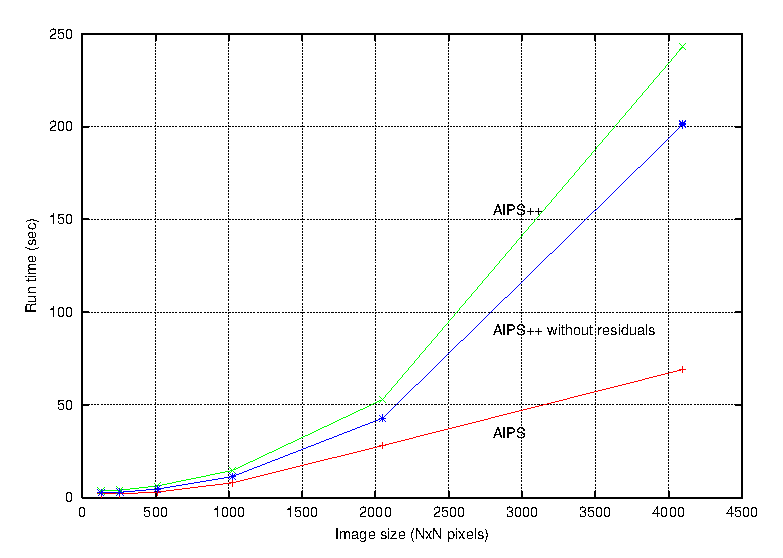
\includegraphics{aips_aips2_I_withoutresidual.2.eps}
\caption[Imaging timing for AIPS and AIPS++]{\small Wall-clock run time for
interferometric imaging in AIPS and AIPS++.  The curve marked {\tt
'AIPS++ without residuals'} represent run time for AIPS++ without
the computation of the final residual image.}
\label{IMAGER_PLOT}
\end{center}
\end{figure}

The tests were done on a 1.7-GHz, 2-CPU, Pentium machine with an L2
cache of 256Kbytes and RAM of 1 Gbytes.  It was ensured that at least
one of the CPUs was not loaded when these tests were done.

The {\tt imager} tool was configured such that for no problem size did
it resort to the Tiled-gridding algorithm (which is significantly
slower)\footnote{See {\tt
http://aips2.nrao.edu/projectoffice/imager.ps} for the latest
status.}.  The maximum usable memory (set in the {\tt .aipsrc}
variable {\tt system.resources.memory}) was set to various sizes
between 1000 and 5000.  The image cache size was set to 500MB.  AIPS++
{\tt imager} was also run by suppressing the residual image
computation.  These numbers are also listed in Table~\ref{IMAGER_TAB}
and plotted in Fig.~\ref{IMAGER_PLOT}.

For problem sizes $\le 2K\times2K$ images, AIPS++ is slower by a
factor of $\sim 1.5$.  For $4K\times4K$ imaging, it is $\sim 3$ times
slower.

The operation of only computing the PSF was also compared for the two
packages.  This we believe largely compares the I/O performance as
applicable to the imaging application.  The data is tabulated in
Table~\ref{PSFTime}, and plotted in Fig.~\ref{PSFPlot}.  The 'new'
AIPS++ timings are after changes in the {\tt ArrayLattice} which now
uses the reference semantics and the changes made in {\tt FFTServer}
and {\tt LatticeConvolver} to remove unnecessary data flips as
detailed in Section~\ref{FFT_CONVOLVE}.  The new AIPS++ timing show
slower divergence from AIPS timing.  Part of the performance
difference possibly comes from a more dynamic memory model used in
AIPS++ as discussed in Appendix~\ref{A:MEM_MODEL}.
%This also shows similar performance
%ratios as the overall imaging benchmark.  Since this test is dominated
%by the difference in the I/O performance of the two packages, it
%suggests that large part of the difference in the performance for the
%full imaging problem is also due to this difference.

\begin{table}[th!]
\begin{center}
\caption{\small Table of wall-clock runtime for the computation of only the
PSF using AIPS and AIPS++.}
\label{PSFTime}
\vskip 0.5cm
\begin{tabular}{|c|c|c|c|}
\hline
PSF size & AIPS timing & AIPS++ timing & AIPS++ timing\\
(Pixels) & (sec)        & (sec)        & New (sec) \\
\hline
128      &  1           &  3.5         & 1.53 \\
256      &  1           &  3.4         & 1.55 \\
512      &  1           &  4.4         & 1.86 \\
1024     &  1           &  6.2         & 2.82 \\
2048     &  4           &  18.6        & 6.48 \\
4096     &  17          &  71.8        & 25.06 \\
\hline
\end{tabular}
\end{center}
\end{table}

\begin{figure}[t!]
\begin{center}
%  \includegraphics[scale=0.9]{makepsf.ps}
  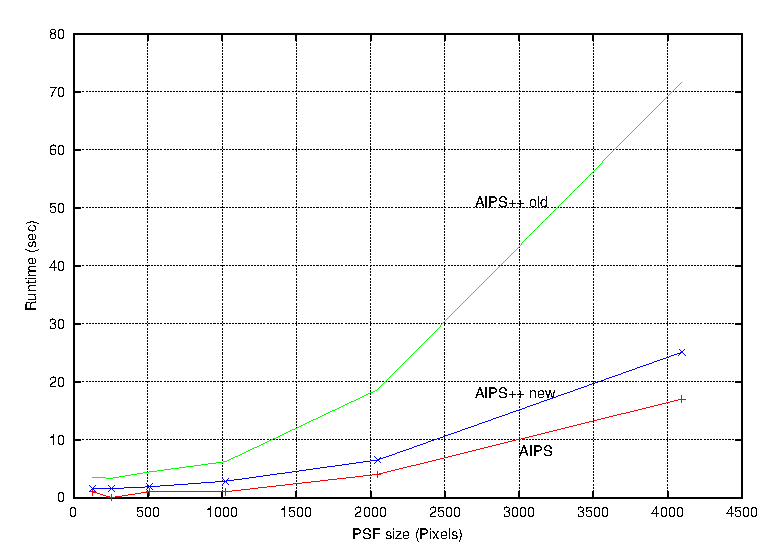
\includegraphics[scale=0.9]{psfonly.time.eps}
\caption[AIPS and AIPS++ time for making PSF only]{\small Wall-clock run time for
making only the PSF using AIPS and AIPS++.  Some of the changes
leading to the {\tt 'AIPS++ New'} curve are detailed in
Section~\ref{FFT_CONVOLVE}.}
\label{PSFPlot}
\end{center}
\end{figure}

For comparison, Fig.~\ref{MIR_AIPS_AIPS++} shows the run time for
imaging in two other acceptable packages, namely AIPS and MIRIAD.  The
AIPS++ curve does not include any attempt at tuning the I/O
performance based on the requirements of the algorithm.  This work is
in progress currently.  Note the diverging performance curves between
AIPS and MIRIAD is not perceived to be a problem by the users.  Out of
the three packages, MIRIAD has the simplest memory model (of fixed
size and limited to the available virtual memory).


\begin{figure}[t!]
\begin{center}
% Original
%\includegraphics[scale=0.5,angle=-90]{aips_aips2_I_withoutresidual.epsi}
  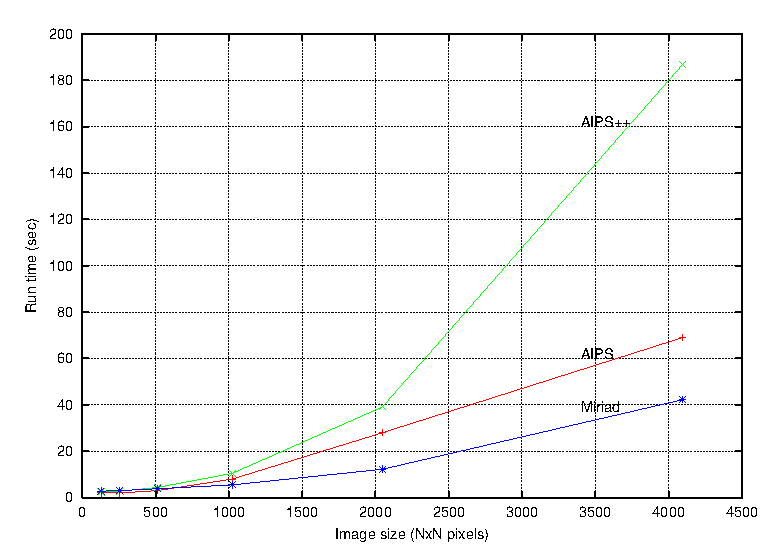
\includegraphics{mir_aips_aips++.imaging.eps}
\caption[Imaging run time comparison between AIPS, MIRIAD and
AIPS++]{\small Wall-clock run time for
interferometric imaging in AIPS, AIPS++ and Miriad.  The AIPS++ curve
includes does not include any attempt at optimizing I/O performance.
Miriad memory model is the simplest (of fixed size and cannot handle
sizes beyond that allowed by the OS).}
\label{MIR_AIPS_AIPS++}
\end{center}
\end{figure}



\subsection{Tiled gridding in AIPS++}

Since the image tile size and cache sizes for the {\tt imager} tool in
AIPS++ can be set at the user level, some tests were done to measure
the performance as a function of these parameters for full stokes
$2K\times 2K$ imaging problem.  This was to test the heuristic that if
the cache size is large enough to hold as many tiles as the number of
visibility points in a single integration, gridding performance will
be optimal.  {\tt imager} was therefore timed for a set of cache size,
tile size and visibility size.  These values are tabulated in
Table~\ref{STOKES_TAB}.

This data suggests that the performance is relatively insensitive to
tile size and the number of visibilities for reasonably large cache
size.  However for smaller cache sizes, it is a stronger function of
the tile size (and possibly of the number of tiles in the cache).

\begin{table}
\begin{center}
\caption{\small Table of AIPS++ timing results for full stokes $2K\times 2K$
imaging using the Tiled gridding mode.}
\label{STOKES_TAB}
\vskip 0.5cm
\begin{tabular}{|c|c|c|c|c|}
\hline
No. of Vis. & Cache size & Tile size & Time     & No. of tiles \\
            & (MBytes)   & (Pixels)  & (sec)    &              \\
\hline
351         &  128       &  2048     & 774      &    04        \\
351         &  128       &  1024     & 784      &    16        \\
351         &  128       &  512      & 774      &    64        \\
351         &  128       &  256      & 777      &   256        \\
351         &  128       &  128      & 716      &  1024        \\
351         &  128       &  64       & 699      &  4096        \\
351         &  128       &  16       & 700      &  65K         \\
            &            &           &          &              \\
351         &  32        &  512      & $\infty$ &   16         \\
351         &  32        &  256      & 745      &   64         \\
351         &  32        &  128      & 822      &  256         \\
351         &  32        &  64       & 1000     & 1024         \\
351         &  32        &  32       & 1446     & 4096         \\
            &            &           &          &              \\
210         &  32        &  1024     & $\infty$ &   04         \\
210         &  32        &  512      & 822      &   16         \\
210         &  32        &  256      & 805      &   64         \\
210         &  32        &  128      & 836      &  256         \\
210         &  32        &   32      & 1133     & 4096         \\
            &            &           &          &              \\
66          &  32        &  512      & $\infty$ &   16         \\
66          &  32        &  256      & 1046     &   64         \\
66          &  32        &  128      & 1208     &  256         \\
66          &  32        &   32      & 1675     & 4096         \\
\hline
\end{tabular}
\end{center}
\end{table}



%%%%%%%%%%%%%%%%%%%%%%%%%%%%%%%%%%%%%%%%%%%%%%%%%%%%%%%%%%%%%%%%%%%%%%%%%%%%%%%%%%%%

\section{I/O Benchmark}
\label{IOBenchmark}

The AIPS++ Table system is the underlying data base management system
which manages data in and out of the disk.  All data related disk I/O
is done using Tables.  It therefore influences almost every data
processing application in AIPS++ and it is important to benchmark the
efficiency of the Table system itself.  However since neither the
AIPS++ Table system's caching/buffering philosophy and the exact
details of the I/O (e.g how it manages the tiles on the disk, provides
random access, sort-order independent access to a multi dimensional
data, etc.) nor such details of AIPS I/O are well understood, this
benchmark was done against, what I refer to as the ``raw UNIX I/O''.
A $N\times4$ array of complex numbers was written to the disk using
the Table system's {\tt DataStMan} and {\tt ShapeStMan} storage
managers as well the raw UNIX {\tt write} call in the native endian
format.  The data written by {\tt write} was read using the UNIX {\tt
read} call while the data written by the Table system was read using
the persistent storage managers (which are committed at the time of
writing the data).  The 'raw I/O' was also buffered and the buffer
size was kept equal to the cache size reported by the Table I/O.  The
``hit rate'' reported by the Table I/O statistics was always $>99\%$.
The timing for this test are tabulated in Table~\ref{IO_TAB}.  For
convenience, the plots of timings and performance ratios are shown in
Figs.~\ref{IOTIME_PLOT} and \ref{IORATIO_PLOT}.  This ratio remains at
$\sim 1.4$ till 4 million rows, rises to $\sim 2$ before it peaks at
$\sim 2.8$ for 8 million rows.  This sudden decrease in the I/O
performance beyond 4 million rows is not well understood.  Also, the
precise cause of the further degradation in the performance for larger
number of rows is unclear as well.  Note that the Table
tile cache size and shape were not varied.  It is the tuning of these
parameters which needs to be explored for optimal I/O performance.

{\it Work to get a better understanding of such issues in I/O
performance is in progress.  To achieve optimal performance, it is
obvious that a deeper understanding of the I/O system by the
application programmers (and the understanding of the application I/O
requirements by the Table system programmers) is crucial. In my
opinion, a more detailed technical document detailing the design, and
recommended usage by the higher level programs is of crucial
importance.}


\begin{table}[h!]
\begin{center}
\caption{\small Table of AIPS++ I/O benchmarks measured against ``raw'' UNIX
I/O.}
\label{IO_TAB}
\vskip 0.5cm
\begin{tabular}{|c|c|c|c|c|c|}
\hline
No. of Rows &UNIX    & DataStMan & ShapeStMan      &DSM/U    & SSM/U  \\
            &[U](sec)& [DSM](sec)& [SSM](sec)      & (Ratio) & (Ratio)\\
\hline 
10000       & 0.01   & 0.01      & 0.01            & 1.0     &1.0     \\
100000      & 0.06   & 0.08      & 0.09            & 1.3     &1.5     \\
1000000     & 0.63   & 0.87      & 0.87            & 1.4     &1.4     \\
2000000     & 1.28   & 1.91      & 1.75            & 1.5     &1.4     \\
4000000     & 2.58   & 5.35      & 3.65            & 2.1     &1.4     \\
6000000     & 3.89   & 6.20      & 6.85            & 1.6     &1.8     \\
7000000     & 4.59   & 7.70      & 7.85            & 1.7     &1.7     \\
8000000     & 5.23   & 11.61     & 14.47           & 2.2     &2.8     \\
%10000       & 0.01  &  0.08 &  0.07 & 8.0 & 7.0 \\
%100000      & 0.09  &  0.75 &  0.68 & 8.3 & 7.5 \\
%1000000     & 0.96  &  7.50 &  6.77 & 7.8 & 7.0 \\
%2000000     & 1.93  & 15.11 & 13.19 & 7.8 & 6.8 \\
%4000000     & 4.75  & 30.60 & 27.31 & 6.4 & 5.8 \\
%6000000     & 6.77  & 46.68 & 40.95 & 6.9 & 6.1 \\
%7000000     & 7.36  & 53.98 & 47.96 & 7.3 & 6.5 \\
%8000000     & 11.59 & 63.41 & 55.28 & 5.5 & 4.8 \\
%9000000     & 10.65 & 69.89 & 62.04 & 6.6 & 5.8 \\
\hline
\end{tabular}
\end{center}
\end{table}

\begin{figure}[h!]
\begin{center}
  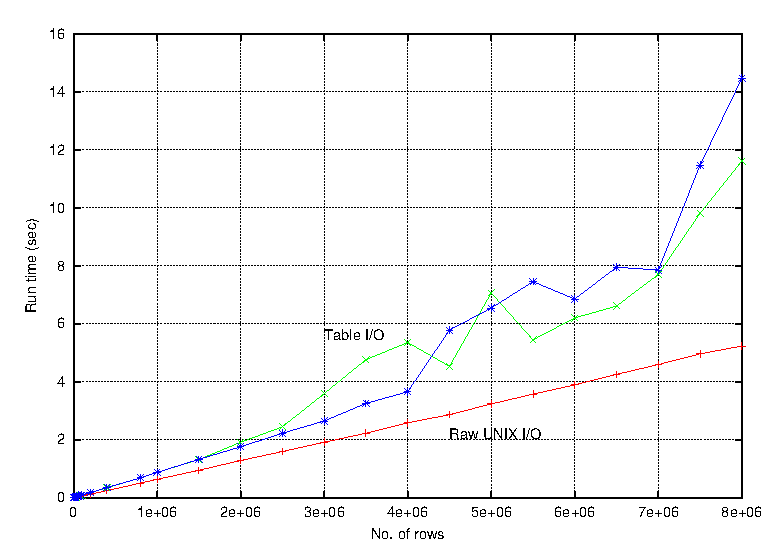
\includegraphics[scale=0.9]{runtime.New.eps}
\caption[AIPS++ and raw UNIX I/O performance]{\small Wall-clock run time
measurements for raw UNIX and AIPS++ Table system I/O as a function of
number of rows in a table of complex numbers.}
\label{IOTIME_PLOT}
\end{center}
\end{figure}

\begin{figure}[h!]
\begin{center}
  \includegraphics[scale=0.9]{ratio.New.eps}
\caption[AIPS++ and raw UNIX I/O performance ratios]{\small Ratio of run time
measurements for raw UNIX vs. AIPS++ Table system I/O as a function of
number of rows in a table of complex numbers.  The two curves
correspond the ratios of DataStMan storage manager (green curve) and
DataShapeStMan storage manager (red curve) with the raw UNIX timing.}
\label{IORATIO_PLOT}
\end{center}
\end{figure}

\section{Benchmarking the {\tt calibrater} tool}

The {\tt calibrater} tools is the primary calibration tool for
interferometric data in AIPS++.  The measured visibility $V$ in AIPS++
is described by the Measurement equation (ME).  It encapsulates the
corruption of the ideal visibilities $V^\circ$ by multiplicative gain
terms (Jones matrices), which in turn can be written as an outer
product of antenna based Jones matrices ($[V]=[J_i \otimes J_j^\star]
[V^\circ]=[J_{ij}][V^\circ]$).  $J$, in general, is a product of
several matrices, each representing a physically independent
corrupting, but solvable term.  In this formulation, the effects of
these multiplicative terms are calibrated by multiplying the observed
visibilities by $J^{-1}$.  Given a set of $N(N-1)/2$ measured and
model complex visibilities ($V$ and $V^M$ respectively), from an $N$
element interferometer, the {\tt calibrater} tool solves for the
various $N$ antenna based Jones matrices ($J_i$s) using a non-linear
least squares (NLLS) iterative algorithm.  As is usual for NLLS
algorithms, starting from an initial guess for the Jones matrix being
solved, the algorithm minimizes $\chi^2 = [V - V^M]^TW[V-V^M]$ in
several iterations, where $W$ is the weights matrix associated with
$V$.  Each iteration computes the update direction by computing
$\partial\chi^2/\partial J_i$ and $\partial^2
\chi^2/\partial J_i\partial J_j$.  The number of iterations required
to reach the solution is a function of the initial guess and the
signal-to-noise ratio in $V$.  Calibrated visibilities are then
computed as $[V^C]=J^{-1} [V]$.

A typical calibration problem involves solving for the (1) {\tt G}
Jones matrix (representing the antenna based complex gains), (2) {\tt
D} Jones matrix (representing the antenna based polarization leakage
gain), and (3) {\tt B} Jones (representing the antenna based,
frequency dependent complex gains).  Solution for these are sought for
one solution interval at a time, where the solution interval is
typically $10-30$s for {\tt G}, and several hours for {\tt D} and {\tt
B}.  Initially, solutions for {\tt G}, using data from the primary
phase and flux calibraters, are sought to phase the array and
establish a flux scale.  Solutions for {\tt B} and {\tt D} are found
using data from potentially separate polarization and bandpass
calibraters.  Later, the {\tt calibrater} tool is used in a
SelfCal loop as well.

Solutions in AIPS++ can be found by first averaging the visibilities
for the entire duration of the solution interval and solving for the
Jones matrices from this averaged visibilities (achieved by setting
{\tt preavg} $=$ {\tt t} in {\tt calibrater.setsolve()}).
Alternatively, solutions can be found by averaging the visibilities
for intervals shorter than solution interval and later averaging these
individual solutions to form an average Jones matrix for the entire
solution interval (achieved by setting {\tt preavg} $<$ {\tt t} in
{\tt calibrater}).  The latter is required for {\tt D} Jones
solutions, but not necessarily required for {\tt G} and {\tt B} Jones
solution.

Since the entire visibility data set is read and written for a full
calibration, the dominant costs for calibration would be a function of
the I/O cost, number of iterations per solution and the entire cost
would scale, close to linearly, as a function of the ratio of {\tt t}
to {\tt preavg} settings for {\tt G} and {\tt D}.  {\tt B} solution is
similar to {\tt G} solution invoked $N_c$ number of times (though with
a longer solution interval) where $N_c$ is the total number of
independent frequency channels.

The solved Jones matrices, as a function of time/ frequency/ IF/
polarization/ ? are stored in Gain Tables, which is a collection of
one slot per solution.  Some additional cost will come from the
overheads of the slot-hunting algorithm.  Ideally, this cost is
expected to be insignificant.

\subsection{Results}

The AIPS++ benchmark tool was used to measure the performance of the
{\tt calibrater} tool.  A 125K visibility per channel, 128 channel
data was simulated for a point source at the phase center.  {\tt G}
and {\tt D} terms were included in the simulation with a ``coherence''
length of 30min and several hours for the two terms respectively.
Same {\tt G} corruption was applied for all frequency channels.  The
calibrater was then run by varying the solution interval to vary the
number of solution intervals from a few to several hundred.  The same
data set was then also used in AIPS and the task {\tt CALIB} used to
derive the equivalent gain tables.  Both process in AIPS and AIPS++
were timed as a function of the number of solution intervals.  The
wall-clock run time is tabulated in Table~\ref{CALIB_TAB} and plotted
in Fig.~\ref{CALIB_PLOT}\footnote{See {\tt
http://aips2.nrao.edu/projectoffice/calibrater.ps} for the latest
updates.}.

In AIPS++, as of now, the {\tt calibrater} tool requires one of the
columns in the MS to be filled in.  The filler does not fill this
column, and one needs to run the {\tt imager} tool to fill this
column.  We noticed that starting {\tt calibrater} before starting
{\tt imager} for this operation, costs $30-40$s of set-up time before
it can start the actual task.  This appears to be related to some
interaction of the Table system's caching/buffering (via the opening
and reading of MS) and the OS caching/buffering (which gets affected
due to an independent process, namely {\tt imager} being started).
The initial high point in the plot includes this extra cost which can
be easily eliminated.

The curve marked {\tt 'Default settings'} (red) in
Fig.~\ref{CALIB_PLOT} is with a run where {\tt preavg} was smaller
than the solution interval.  As one can see, the run time rises,
approximately linearly, with the number of solution intervals.  Just
for the test, switching off the slot-hunting algorithm in the tool
generates the curve marked {\tt'No slot-hunting'} (green).  The
difference between these two curves is the cost of slot-hunting
algorithm.  This clearly needs to be optimized further.  Setting {\tt
preavg} equal to the solution interval for {\tt G} Jones solution
generates the curve marked {\tt 'preavg=Solint'} (blue).  This
suggests that by default, {\tt calibrater} tool should be configured
with {\tt preavg} set equal to the solution interval, at least for
{\tt G} and {\tt B} solutions.  It needs to be different for {\tt D}
solution and that should be explicitly set.

The issue of {\tt 'preavg=Solint'} has now been fixed (see also the
progress report on {\tt calibrater} improvements on AIPS++ Project
Office) by working with the nominal point-source visibilities, now
correctly computed as $\frac{\langle V^{Obs} V^{{Cor}^\star}
\rangle}{\langle |V^{Cor}|^2
\rangle}$ where $V^{Obs}$ is the uncorrected observed data and
$V^{Cor}$ is the model data corrupted by the estimated Jones
matrices.  This eliminates the need for the extra
{\tt preavg} parameter for {\tt G} and {\tt B} solutions.  However it
is still required for {\tt D} solutions.

The AIPS run time (not plotted on the graph in Fig.~\ref{CALIB_PLOT})
was surprisingly flat at $\sim10$s.  At this stage we do not
understand this behavior, since fundamentally, any algorithm needs to
do more work, and hence take longer, as a function of the number of
solution intervals.  A possible explanation for such a flat curve
could be that AIPS manages to hold the selected data in memory (and
the OS retains those buffers from one run to the other since the
machine was not loaded otherwise).  This can eliminate the time
required to read the data from the disk.  Also, the {\tt G} and {\tt
D} corruptions in the simulated data are flat as a function of time,
within the coherence length.  This means that if the solution found
for a solution interval is passed on as the initial guess for the next
solution interval, the number of iterations can be sharply cut down
(and may be completely eliminated for most solution intervals for the
current simulated dataset).  We do not know if this is affecting the
AIPS timings at this stage.

\begin{figure}[h!]
\begin{center}
  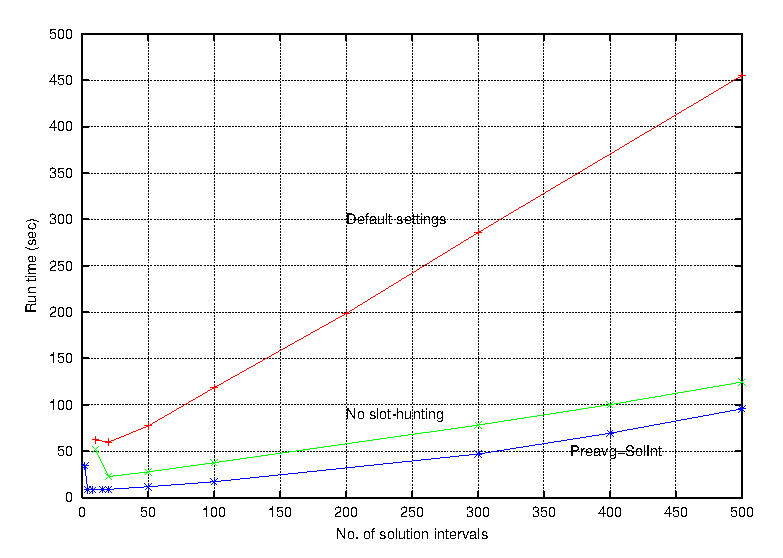
\includegraphics[scale=0.9]{calib.ps}
\caption[AIPS++ {\tt calibrater} performance]{\small Plot of {\tt calibrater}
wall-clock run time as a function of number of solution intervals.}
\label{CALIB_PLOT}
\end{center}
\end{figure}

It is not simple to run the AIPS task {\tt CALIB} to solve for
variable number of channels.  A comparison between AIPS and AIPS++ for
{\tt B} solution as a function of number of channels was therefore not
done.  The AIPS++ performance curve is however shown in
Fig.~\ref{BP_PLOT}.  We feel that passing the solutions for one
channel as the initial guess for the next channel may have significant
impact in run time for this case\footnote{See {\tt
http://aips2.nrao.edu/projectoffice/calibrater.ps} for performance
improvement when this is done.}, since typically, bandpass calibration
curve is a slowly and smoothly varying function of channel.  The
solution from one channel will be a very good initial guess for the
next channel and the convergence will be faster.

\begin{table}[h!]
\begin{center}
\caption{\small Table of AIPS++ vs. AIPS calibration run time for {\tt G}
Jones solutions. Third column lists the wall-clock run time for AIPS++
in it's current, default configuration.  Fourth and fifth columns are
the run times after suppressing slot-hunting algorithm and setting
{\tt preavg} equal to solution interval respectively.}
\label{CALIB_TAB}
\vskip 0.5cm
\begin{tabular}{|c|c|c|c|c|c|}
\hline
No. of slots& AIPS &     AIPS++    &         AIPS++        &    AIPS++\\
            & (sec)& [default](sec)& [no slot-hunting](sec)& [preavg](sec)\\
\hline
10          &  11  &     62.3      &         51.9          &  8.7 \\
20          &  11  &     59.7      &         22.7          &  8.9 \\
50          &  11  &     77.3      &         27.7          & 11.7 \\
100         &  10  &    118.5      &         37.6          & 17.0 \\
200         &  10  &    198.4      &         78.2          &  -   \\
300         &  10  &    285.7      &        100.1          & 46.9 \\
500         &  10  &    455.0      &        124.6          & 95.7 \\
\hline
\end{tabular}
\end{center}
\end{table}
\begin{figure}[!h]
\begin{center}
  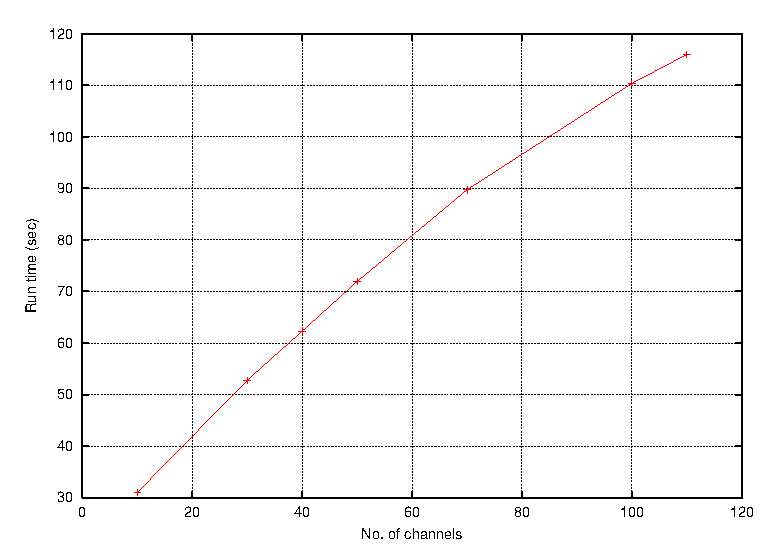
\includegraphics[scale=0.9]{BPTime.ps}
\caption[AIPS++ {\tt calibrater} performance for {\tt B}Jones]{\small Plot of
{\tt calibrater} wall-clock    run time as a  function    of number of
frequency channels.}
\label{BP_PLOT}
\end{center}
\end{figure}

\section{FFT and Convolutions}
\label{FFT_CONVOLVE}

Profiling of {\tt imager} showed that the application spent maximum
fraction of time in the {\tt Copy::objcopy()} method.  This method is
used to copy data between memory buffers and all these calls were
triggered either in the Table system or in the {\tt FFTServer} (via
the {\tt LatticeConvolver::convolve() ->} {\tt LatticeFFT::fft() ->}
{\tt FFTServer::fft() ->} {\tt FFTServer::fft0() ->} {\tt
FFTServer::flip() ->} {\tt Copy::objcopy()} chain).  We therefore
examined {\tt FFTServer} with the goal of minimizing memory copies if
possible.

AIPS++ uses the {\tt FFTPACK} library for the various versions of the
FFT algorithm (Real{\tt->}Complex, Complex{\tt->}Complex,
Complex{\tt->}Real).  {\tt FFTServer} is the C++ wrapper class which
provides these FFT services.  Images are represented using the {\tt
TempLattice} classes, which in turn are derived from the {\tt Lattice}
base class and uses the {\tt ArrayLattice} if the desired image fits
in the available memory or {\tt PagedArray} if the available memory is
not sufficient.  The decision about the available memory is controlled
by the {\tt .aipsrc} variable {\tt system.resources.memory}.

FFT and FFT based convolution operations on images are done via the
{\tt LatticeFFT} and {\tt LatticeConvolver} classes respectively.  As
mentioned in Section~\ref{IMAGER}, FFT is used once for making the
PSF, and then in every Clark Clean major cycle via the convolution for
making the model visibilities.  Convolution of the PSF with the CC
model is done via the following operations:

\begin{enumerate}

\item Flip the PSF, take the FFT to make the transfer function (XFR)
and flip the XFR back again
\label{F1}

\item Flip the CC image, take the FFT ($V$), and flip the
result again
\label{F2}

\item multiply the XFR with $V$, flip the result, do an inverse
FFT and flip the result again
\end{enumerate}

The flipping operation is a circular shift of the functions along each
axis by N/2 pixels where N is the size of the image along an axis.
Flipping an image via a call to {\tt FFTServer::flip()} costs $O(3N)$
calls per axis to {\tt Copy::objcopy()}.  The FFT algorithm expects
the origin of the function along each axis to be located at the first
pixel along each axis - often referred to as the {\it flipped order}.
Functions (images in our case) represented in the {\it natural order}
have their original located at $N/2$.  Without the flipping operation,
the Fourier transform of a function $I$ is given by
\begin{equation}
I(x,y)~ \rightleftharpoons ~ V(u,v) e^{-2\pi\iota\left[u N_x/2 + v N_y/2\right]}
\end{equation}
where $N_x$ and $N_y$ are image sizes along the two axis and $V$ will
be in the flipped order.

The flipping operation on $I$ eliminates the extra phase term in the
Fourier domain.  For the purpose of convolution then, it is sufficient
to flip the PSF only.  Without the flips in Step~\ref{F2}, $V$ will
carry the phase term.  Complex point-by-point multiplication of XFR
with $V$ will ensure that after taking an inverse Fourier transform,
the resultant convolution will be in the natural order.  This reduces
the number of flips to only $O(N)$ per axis of the PSF, and is
independent of the number of convolutions (provided, of course, the
transfer function does not change!)\footnote{The flipping operation
can also be implemented as a phase ramp in the conjugate Fourier
domain.  For even sized images, this translates to flipping the sign
bit of every other pixel.  See
http://aips2.nrao.edu/projectoffice/imager.ps for performance
improvements due to this.}.

%\subsection{The changes (this section is really for personal notes!)}

%The following pseudo code details the changes made in {\tt
%LatticeConvolver}, {\tt LatticeFFT} and {\tt FFTServer}.

%\begin{verbatim}
%LatticeConvolver::convole
%  LatticeFFT::rcfft  [In size: NxN]
%  Multiply
%  LatticeFFT::crfft  [Out size: NxN]



%LatticeFFT::rcfft    [In: NxN, Out: ]
%  LatticeFFT::rcfft
%    if (doShift)                                 |
%      FFTServer::fft [In: NxN, Out: ]            |
%        Flip --> FFT --> Flip                    | R -> C
%    else                                         |
%      FFTServer::fft0()                          |
%        FFT                                      |

%    if (doShift)                                 |
%      FFTServer::fft(doFlip==1) [In: NxN, Out: ] |
%        if (doFlip==1) Flip                      |
%         FFT                                     | C -> C
%        if (doFlip==2) Flip                      |
%    else                                         |
%      FFTServer::fft0()                          |
%        FFT



%LatticeFFT::crfft   [In (N/2+1)xN, Out: ]
%  LatticeFFT::crfft(another version)
%    if (doShift)                                       |
%      FFTServer::fft(doFlip=2)  [In: (N/2+1)xN, Out: ] |
%        if (doFlip==1) Flip                            |
%        FFT                                            | C -> C
%        if (doFlip==2) Flip                            |
%    else                                               |
%      FFTServer::fft0                                  |
%        FFT                                            |

%    if (doShift)                                       |
%      FFTServer::fft(doFlip=2)  [In: (N/2+1)xN, Out: ] |
%        if (doFlip==1) Flip                            |
%        FFT                                            | R -> C
%        if (doFlip==2) Flip                            |
%    else                                               |
%      FFTServer::fft0                                  |
%        FFT                                            |



%LatticeConvolver::makeXfr  [In: NxN, Out: (N/2+1)xN]
%  LatticeFFT::myrcfft
%    FFTServer::myfft(doShift=True)
%      if (doShift) FFTServer::myfft()      Flip->FFT   | R -> C
%      else         FFTServer::fft0()       Only FFT    |
%      if (doShift) FFTServer::fft(doFlip=1) Flip->FFT  | C -> R
%      else         FFTServer::fft0          Only FFT   |
%\end{verbatim}

%This ultimately achieves the following during convolution:

%\begin{verbatim}
%   f1:  Flip --> FFT ---------+
%                               \
%                                \
%                                 X---> FFTInverse (f1*f2)
%                                /
%                               /
%   f2:           FFT ---------+
%\end{verbatim}	

\subsection{The {\tt FFTW} library}

2D FFTs are realized by performing the appropriate 1D FFTs along the
two axis.  Data for each row (or column) is copied into a contiguous
buffer, and the Fourier transform of this buffer is copied back into
the row (or column).  For a NxN image, this requires 4N
memory-to-memory copies.  It is hoped that with the data for 1D FFT
available in a contiguous buffer, cache misses will be minimized.
However, processor caches are usually much smaller than the typical
size of 1D FFT encountered in AIPS++.  Clearly, cache misses will not
be optimal.

FFTW library provides a FFT complier, optimizer and a scheduler for
computers with hierarchal memory model (smaller but faster L1/L2
caches, larger but slower RAM, and even larger and slower virtual
memory).  It works by first determining a range of sizes of the FFT
butterfly network which will execute fastest on a given processor
(essentially from the faster cache) and then generate an efficient
{\it code-let} for it.  It then determines the {\it plan} to decompose
a given FFT problem into smaller problems (i.e., smaller FFT butterfly
sub-nets).  The {\it codelet} of these smaller problems, the data for
which fits in the cache, are then scheduled for execution.  It can be
shown\footnote{See FFTW: An Adaptive Software Architecture for the
FFT; Frigo, M. \& Johnson, S. G., 1998, ICASSP conference proceedings,
Vol. 3, pp. 1381-1384 and {\tt http://www.fftw.org}} that this
strategy minimizes the number of cache misses (asymptotically
approaching the theoretical value) and the execution speeds are
comparable to those given by implementations specifically tuned for
certain processors.  Since FFTW library generates the {\it plan} at
runtime and makes no assumption about the cache size, cache length,
etc., it is a cache-oblivious algorithm and hence portable.

For AIPS++, use of FFTW library in {\tt FFTServer} will certainly
eliminate the remaining calls to {\tt objcopy} in the inner loops and
may optimize cache misses (at least for cases which can be handled in
RAM).  {\it Note also that once FFTW is in use, it is relatively
simple to use the threaded versions of FFT which should further
improve the performance on the ubiquitous multi-cpu computers
available these days}.  Table~\ref{FFT_TAB} shows the comparative
performances of the {\tt FFTPACK} and the FFTW libraries for an
in-place, complex-to-complex 2D FFT.  The AIPS++ {\tt TempLattice} was
used to hold the images entirely in the memory (i.e., no {\tt
PagedArray}.  See Appendix~\ref{A:PAGED_FFT} for more complicated
situations using OS swapping and {\tt PagedArray}s).  The data is
plotted in Fig.~\ref{FFT_PLOT}.  The test was done on a 1.6 GHz CPU
with 512 KB L2 cache and 512 MB of RAM.  The test was run a number of
times to account for unpredictable (small) changes in the wall-clock
run time.  FFTW was consistently faster by at least a factor of $2$.
Note that image sizes which are composite of 2, 3 or 5 ($N=2^p 3^q
5^r$ where $p,q,r$ are integers $\ge 0$) are also included.  With the
default setting in {\tt imager}, we do a 20\% padding and use the
nearest size after padding which is a composite of 2,3 or 5.

\begin{table}[h!]
\begin{center}
\caption{\small Table of wall clock run time for a complex-to-complex 2D FFT
test using {\tt FFTPACK} and {\tt FFTW} libraries.}
\label{FFT_TAB}
\vskip 0.5cm
\begin{tabular}{|c|c|c|}
\hline
Image     & FFTPACK &  FFTW   \\
size(NxN) & (sec)   & (sec)   \\
\hline
128       & 0.01    & $<0.01$ \\
256       & 0.06    & 0.01    \\
512       & 0.29    & 0.13    \\
600       & 0.18    & 0.09    \\
1024      & 1.23    & 0.58    \\
1250      & 0.81    & 0.54    \\
1296      & 0.85    & 0.42    \\
1440      & 1.14    & 0.59    \\
1600      & 2.67    & 1.11    \\
2000      & 2.18    & 1.32    \\
2048      & 4.77    & 2.46    \\
2430      & 3.80    & 1.91    \\
3000      & 6.50    & 3.57    \\
3456      & 13.92   & 6.87    \\
4096      & 22.23   & 10.51   \\
4860      & 30.66   & 11.41   \\
\hline
\end{tabular}
\end{center}
\end{table}

\begin{figure}[h!]
\begin{center}
  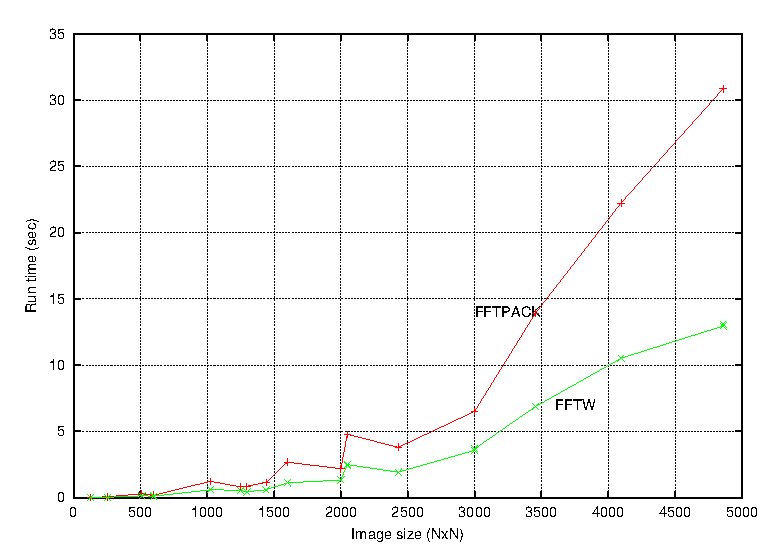
\includegraphics[scale=0.9]{ffttime_langur.eps}
\caption[FFTPack vs FFTW performance for 2D FFTs]{\small Plot of the
wall-clock run time as a function of the 2D image size using the
FFTPack and FFTW libraries.}
\label{FFT_PLOT}
\end{center}
\end{figure}

\newpage
\appendix{}


\section{Appendix}
\subsection{Large sized FFT}
\label{A:PAGED_FFT}

Images in AIPS++ are represented using {\tt TempLattice}.  The maximum
usable memory is specified via the {\tt aipsrc} variable and image
sizes which do not fit in the memory are represented using the
underlying {\tt PagedArray} classes.  Of particular interest would be
the impact on the performance due to interaction (if any) between OS
and AIPS++ paging, using large image sizes.

Fig.~\ref{LARGE_FFT_PLOT} shows the wall-clock timing as a function of
image sizes, with the maximum usable memory set to 20/50, 100 and
500MB (on a machine with 512MB RAM).  The curves for 500MB memory
model look similar to the one in Fig.~\ref{FFT_PLOT}.  AIPS++ paging
(via {\tt PagedArray}) kicks-in for image size of $2000\times2000$ for
50MB and at $2430\times2430$ for 100MB models.  At this stage, there
is no performance gain in going to FFTW.  If the images were entirely
held in the memory, OS swapping would start between the image sizes of
3000-4000.  It is curious that there is a significant drop in the
performance around these problem sizes.  The reasons for this are
unclear but suggests that the {\tt TempLattice::niceCursorShape()}
method could be made OS virtual memory aware (or should we say {\tt
virtual-memory-oblivious}!! $\smile$).


\begin{figure}[h!]
\begin{center}
  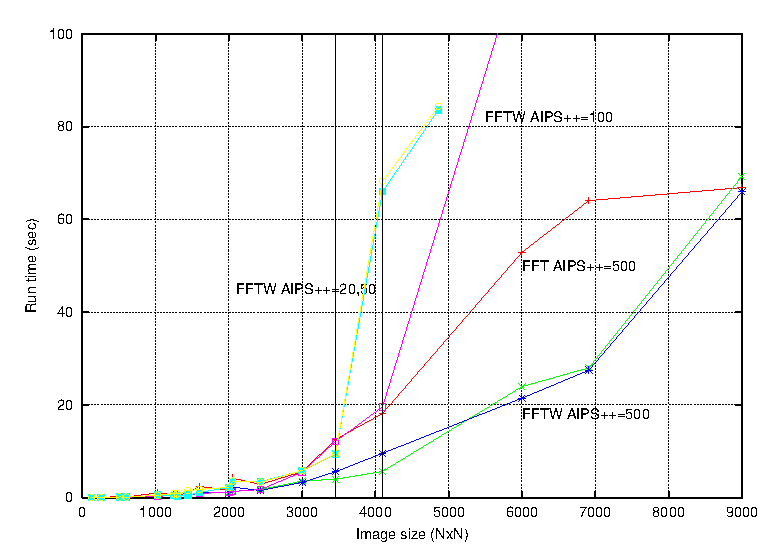
\includegraphics[scale=0.9]{fft_time.eps}
\caption[FFTPack vs FFTW performance for 2D FFTs for larger sized
images]{\small Plot of the wall-clock run time as a function of the 2D image
size using the FFTPack and FFTW libraries.  Curves marked {\tt
'AIPS++=500'} and {\tt 'AIPS++=100'} were generated with the
maximum usable memory set to 500MB and 100MB (on a 512MB RAM machine)
respectively.  The ones marked {\tt 'AIPS++=20,50'} were with the
settings of 20MB and 50MB respectively and the performance was similar
for these cases. {\tt PagedArray} gets used for $N \ge 2000$ and $N
\ge 2430$ for the 50MB and 100MB cases respectively.  The two vertical lines
indicate the approximate sizes where OS swapping starts.}
\label{LARGE_FFT_PLOT}
\end{center}
\end{figure}

\subsection{Memory usage}
\label{A:MEM_MODEL}

It is difficult to compute the maximum required memory for the
execution of a given problem size using {\tt imager}.  The run time
memory and CPU usage for a typical run of {\tt imager} was therefore
monitored and is plotted in Fig.~\ref{MEM_CPU_USAGE}.  Curves for the
total in-core memory and the data memory are always close to each
other implying that most of the data required by the program at all
times is in the RAM.  There is wide fluctuation in the required memory
as the program executes and corresponding fluctuation in the CPU
usage.  Fluctuation in memory usage appears to imply a large number of
kernel calls to allocate and release memory buffers.  The integrated
impact of this on the overall performance is unclear (simple tests
suggest that there is significant cost associated with frequent kernel
calls for memory management).  For comparison, the AIPS runtime memory
usage profile is remarkably featureless - for the same problem, it
quickly reaches $\sim 25MB$ and stays put there for the entire
lifetime of the process.

\begin{figure}[h!]
\begin{center}
  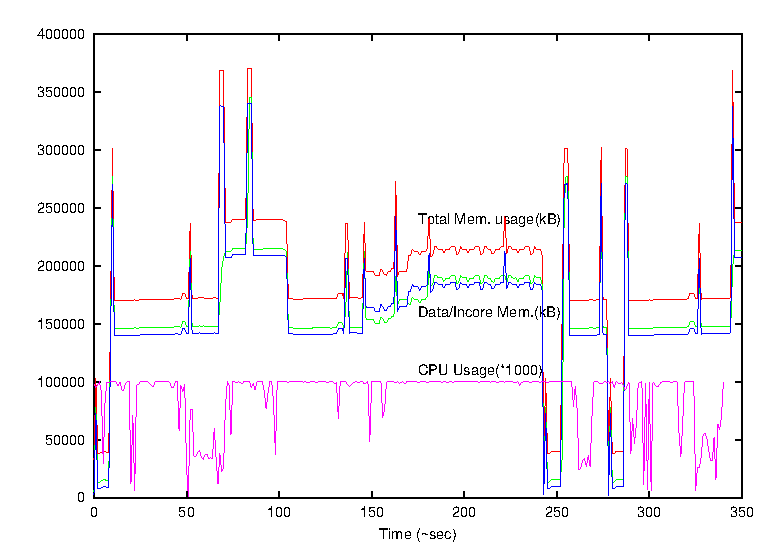
\includegraphics[scale=0.9]{mem_cpu_usage.ps}
\caption[Runtime memory and CPU usage of {\tt imager}.]{\small Plot showing
the runtime memory and CPU usage of {\tt imager}.  The units along the
y-axis are Kilobytes.}
\label{MEM_CPU_USAGE}
\end{center}
\end{figure}

{\it The memory model used in AIPS++ is reasonably configurable via
user defined parameters (though there are places in the code where the
maximum available size is hard coded).  However, in the default
settings shipped with the current AIPS++ distribution, this model is
rather conservative for most machines on which AIPS++ now runs.
Changing these parameters to reflect a larger memory model and making
these parameters aware of the RAM size/number of CPUs available will
be most useful.  Eliminating any hard coded numbers in the code
controlling the memory model should almost certainly be done (e.g.,
the code for {\tt LatticeConvolver}, which constitutes a major
compute-cost during deconvolution, has a burnt-in number assuming a
RAM size of 64MBytes).}

\section{Appendix: Tools and Techniques}
\subsection{Profiling AIPS++ using {\tt gprof}}
\label{A:GPROF}

Most high level application programs in AIPS++ (like {\tt imager} and
{\tt calibrater}) use large parts of the base libraries.  First step
towards improving the performance of such applications involves
locating the performance hot-spots.  Such hot-spots in a large
software system can arise due to a variety of reasons including
genuine bugs, inefficient use of lower level classes, algorithmic
bottle-necks, etc.  Locating the precise section(s) of the code where
the application spends the majority of its time involves instrumenting
the application code with stubs.  These stubs typically {\it estimate}
the fraction of the total runtime that was spent in each of the
methods of the various classes used.  Instrumenting the binary code is
done either by commercially available tools or by tools like the {\tt
``-pg''} option of {\tt gcc/g++/g77} in conjugation with tools like
{\tt gprof}.  Most of the work described in this note was done using
these GNU tools.

Profiling AIPS++ an application involves two steps.  First, the parts
of the code that needs to be profiled must be compiled with the {\tt
``OPT -pg''} options of {\tt gcc/g++}.  {\tt OPT} here refers to the
compiler optimization flags (which usually is equal to {\tt ``-O2''}).
Including this option is important since the resulting runtime profile
will include all the compiler level optimization.  Without this, the
real performance hot-spots may get obscured by the code which is
otherwise automatically optimized by the compiler.  The `{\tt ``-pg''}
option instruments the code.  Note that {\it all} parts of the
code-base, including the object code in the AIPS++ libraries which
requires examination for performance improvements, needs to be compiled
with these options.

Running an application compiled with the {\tt ``-pg''} option
generates a file named {\tt ``gmon.out''} in the local directory.
This file contains the information about the runtime profile of the
application.  The {\tt gprof} program then converts this information
into a human readable call-tree with the estimated total and
fractional time spent in each method and its children (this, for a
full AIPS++ profile is a large file).  Note that since {\tt all}
profiled applications automatically create the file named {\tt
``gmon.out''}, running multiple instrumented AIPS++ distributed
objects from {\tt glish} will overwrite this file (and possibly
corrupt it).

The output of {\tt gprof} is split into two sections - the {\tt Flat
profile} and the {\tt Call graph} sections.  The {\tt Flat profile}
section is a table of columns containing information about the various
methods which were executed and the fraction of the total time spend in
each of them.  The table contains the following columns (the following
table is the last thing in the {\tt Flat profile} section!):

\begin{verbatim}
 %           the percentage of the total running time of the
time         program used by this function.

cumulative   a running sum of the number of seconds accounted
 seconds     for by this function and those listed above it.

 self        the number of seconds accounted for by this
seconds      function alone.  This is the major sort for this
             listing.

calls        the number of times this function was invoked, if
             this function is profiled, else blank.
 
 self        the average number of milliseconds spent in this
ms/call      function per call, if this function is profiled,
             else blank.

 total       the average number of milliseconds spent in this
ms/call      function and its descendents per call, if this
             function is profiled, else blank.

name         the name of the function.  This is the minor sort
             for this listing. The index shows the location of
             the function in the gprof listing. If the index is
             in parenthesis it shows where it would appear in
             the gprof listing if it were to be printed.
\end{verbatim}

The {\tt Call graph} section is a detailed call graph, starting from
the top-level method in which the application spent most of its time
(the {\tt main()}!).  Every function/method call in this section is
labeled by a unique number printed within square-brackets ({\tt []} -
these are the only places where square-brackets are using the output).
The number within these brackets in the left-most column is the tag
for the function call with which it is associated.  The call-graph of
each function is a list of child function calls made by the function.
Each child-function is further tagged by a number in square-brackets,
which appear immediately after the name of the child-function.  Hence,
one can quickly traverse a particular branch of the call-graph by
repeatedly searching for these tagged numbers in a text editor.  A
graphical tool {\tt kprof} is also freely available for viewing the
call-graph - but it was found to be unstable, at least for large
profiles like those produced by AIPS++ applications.

A possible way to wade through this potentially large amount of
information is to start with the most expensive calls from the top of
the {\tt Flat profile} and follow their call graphs to locate the
children in which inordinate amount of time was spent.

Profiled versions of the entire AIPS++ libraries is usually built on
{\tt atlas}. 


\subsection{Monitoring memory usage}
\label{A:MEMUSAGE}

AIPS++ dynamic memory usage model is quite flexible.  This has the
advantage that the applications can fine tune the memory usage well,
but also has the disadvantage that it can also be easily used in an
non-optimal fashion.  Runtime memory usage monitoring was found to be
a useful diagnostic for possible problems.  Runtime memory usage
profile in conjugation with even a rough idea of the maximum memory
requirements of an algorithm can be an effective way of homing on to
one kind of performance bottle-neck.  The script given below was used
during most of this work to monitor the memory usage.  This script
works on Linux flavored Unixes.  Given the name of the executable
who's memory usage needs to be monitored, it finds the PID, and
extracts the required information from the {\tt /proc/<PID>/status}
virtual file system of Linux.  The application name to be monitored,
the output file name and the sampling time are provided as
command-line arguments.  Apart from a lot of other information in the
output file, {\tt VmSize}, {\tt VmData} and {\tt VmRSS} tags give the
total virtual memory size, the size of data section of the memory and
the total resident memory of the application in kilobytes.  Each
sample in the output file is separated by the output of the {\tt date}
command.

\begin{verbatim}
#! /bin/bash 
#
# 1st arg: Name of the process to monitor
# 2nd arg: output file name
# 3rd arg (optional): Sampling time (sec) 
#   (This is the arg to the 'sleep' command.  For finer than a 
#    second sampling, use 'usleep')
#

if [ $# -lt 2 ]
then 
  echo "Usage: " `basename $0` \
       " <Process name> <output file> [sampling time (sec)]";
  exit;
fi

SAMPINTERVAL='1';
echo -n "Looking for process '"$1"'..."
pid=''
while(test -z $pid)
do
 pid=''
 pid=`ps -elf | grep $USER | grep $1 | grep -v grep | \
      grep -v memusage|awk '{print $4}' -`
done

echo "..got the PID ("$pid").  Starting recording..."

if [ $# -ge 3 ]
then
 SAMPINTERVAL=$3;
fi

date >| $2;
while(true) 
do 
  cat /proc/$pid/status >> $2 ;
  sleep $SAMPINTERVAL;
  date >> $2;
done
\end{verbatim}


%\section{Appendix}
\subsection{Open questions}
\label{A:QUESTIONS}

\begin{enumerate}
\item {\tt TempLattice::init()}

When in the disk based mode, each construction of {\tt TempLattice}
results into a creation of a Table on the disk.  {\tt
TempLattice::init()} gets called twice in each call to {\tt
LatticeConvolver::convolve()}, which in turn is called in the inner
loop of Clark-CLEAN.  When {\tt TempLattice} uses {\tt PagedArray},
this results into creation of a new Table every time.  {\bf Is this a
performance hit?}

\item What's the design/functional/whatever advantage in the
LatticeFFT layer?  Should LatticeFFT be just derived from FFTServer
and LatticeConvolver be part of LatticeFFT (or at least derived from
it)?  Use of the two other convolves in AIPS++ (the {\tt Convolver}
class and the {\tt StokesImageUtil::convolver} should certainly be
discouraged.

%\item {\tt Copy::objcopy()} vs. Macro

%A comparision between a function call to {\tt Copy::objcopy()} and a
%'call' to a macroized version of {\tt objcopy()} reveals that with GCC
%3.1.1, the latter is 3-4 times faster than the former.  The exact code
%used for this test is listed in Appendix~\ref{OBJCOPY}.  The program
%was run several time to account for the changes in timing from
%run-to-run.  Some typical numbers for 100000 transpose of a $128\times
%128$ image are:

%\begin{verbatim}
%   Function:   125.47 real   125.52 user    0 system
%   Macro:       32.34 real    32.33 user    0 system

%   Function:   128.19 real   128.19 user    0 system
%   Macro:       36.27 real    36.27 user    0 system

%   Function:   156.04 real   156.06 user    0 system
%   Macro:       37.71 real    37.71 user    0 system
%\end{verbatim}

%In a typical run of {\tt imager} ($\sim64$K visibilities, $2K\times2K$
%continuum, total intensity imaging), we incur $\sim300,000$ calls to
%{\tt objcopy()}.


\end{enumerate}

\end{document}


1.

Ger van Diepen writes:
 > Sanjay,
 >
 > I've purified tLatticeIterator and found a leak.
 > I guess this leak is the same as the one in imager.
 >
 > I've fixed LatticeIterInterface.cc and checked it in.
 > Purify shows no leak anymore.
 >
 > The leak was very stupid and made absolutely no sense.
 > There was a needless getStorage in setCurPtr2Cursor which I've removed now.
 > So apart from fixing the leak you should also get performance
 > improvement because that getStorage took about 35% of all
 > getStorage time (according to your profile).
 > If you want to see it, look for setCurPtr2Cursor in the profiler
 > output.
 >
 > If you profile again (with this fix), setCurPtr2Cursor should not
 > appear anymore in combination with getStorage.
 >
 > Maybe it is a good idea to measure the performance improvement of
 > my Array change and this change in separate runs, so we can see what
 > the effect of each of them is.
 >
 > Cheers,
 > - Ger
 >

2.

Lattice/Array classes memory management needs a serious review?
